\subsubsection{Gestão de unidades curriculares}

Na pagina de gestão de unidades curriculares, um docente pode consultar todas as unidades curriculares em que este está inserido (figura ~\ref{fig:teacher_ucs_index}) e criar uma nova unidade curricular (figura ~\ref{fig:teacher_new_uc}).


\begin{figure}[H]
  \centering
  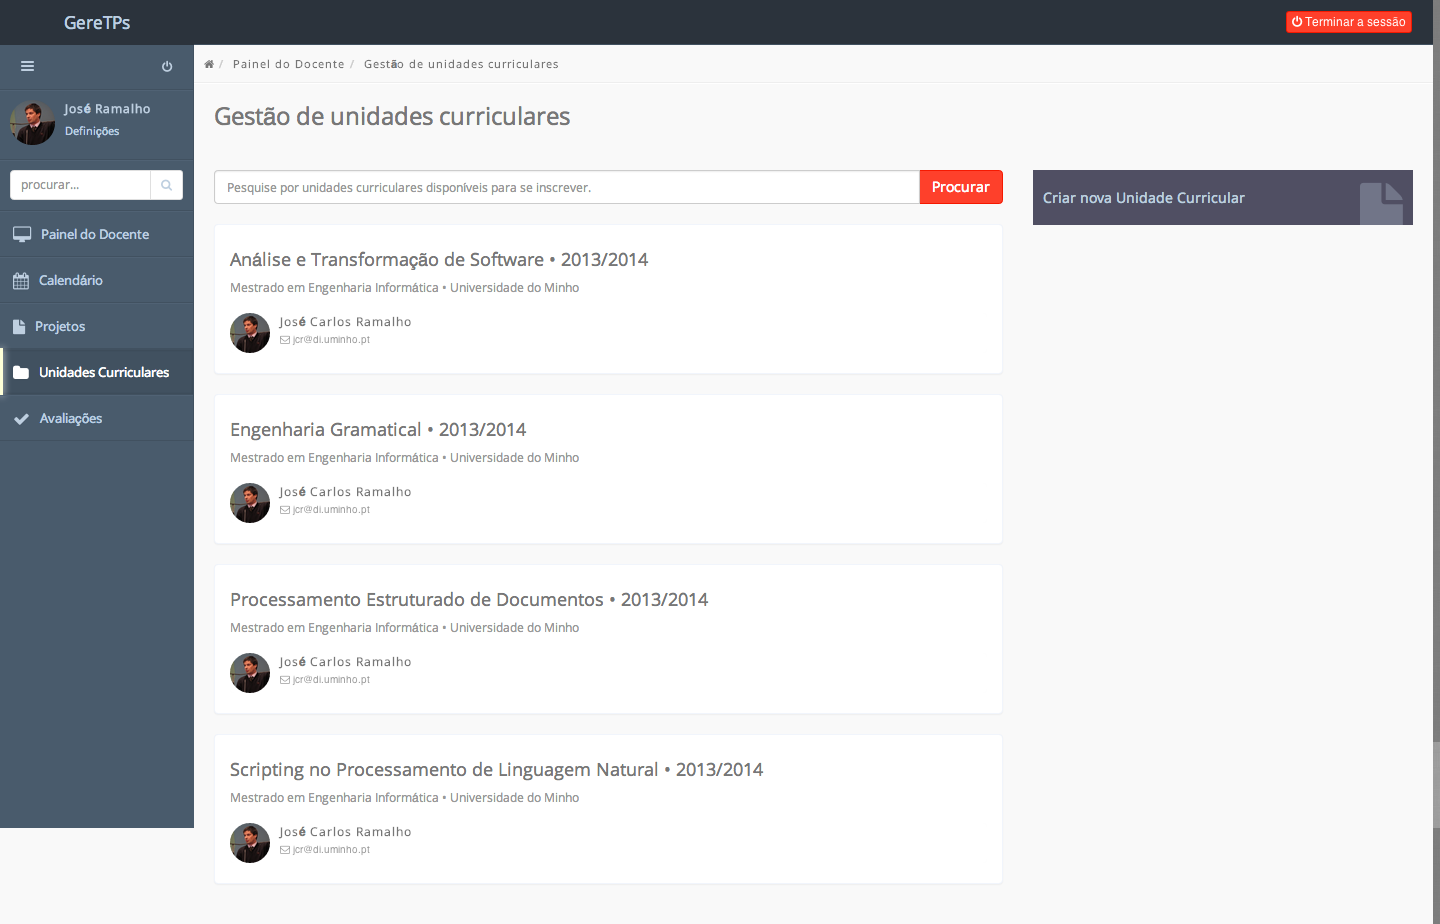
\includegraphics[width=1\textwidth,center]{images/implementacao/docentes/ucs_index}
  \caption{Página de gestão de unidades curriculares}
  \label{fig:teacher_ucs_index}
\end{figure}

\begin{figure}[H]
  \centering
  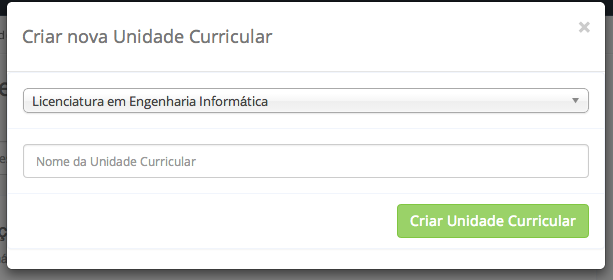
\includegraphics[width=1\textwidth,center]{images/implementacao/docentes/new_uc}
  \caption{Nova Unidade Curricular}
  \label{fig:teacher_new_uc}
\end{figure}

Após criar uma nova unidade curricular, o docente é reencaminhado para a página da unidade curricular criada.

Na página de uma unidade curricular é possível visualizar os projetos dessa unidade curricular, adicionar docentes e fazer gestão de alunos e turnos.

Na página de gestão de alunos (figura ~\ref{fig:uc_students}), um docente pode aceitar ou remover a inscrição de um aluno.

\begin{figure}[H]
  \centering
  
\includegraphics[width=1\textwidth,center]{images/implementacao/docentes/uc_students}
  \caption{Gestão de alunos de uma unidade curricular}
  \label{fig:uc_students}
\end{figure}


Na página de gestão de alunos (figura ~\ref{fig:uc_shifts}), um docente pode criar turnos e adicionar ou remover um aluno de um turno.

\begin{figure}[H]
  \centering
  \includegraphics[width=1\textwidth,center]{images/implementacao/docentes/uc_shifts}
  \caption{Gestão de turnos de uma unidade curricular}
  \label{fig:uc_shifts}
\end{figure}


Na Figura~\ref{fig:teacher_subjects} pode ser consultada uma imagem demonstrativa da página desenvolvida.

\begin{figure}[H]
  \centering
  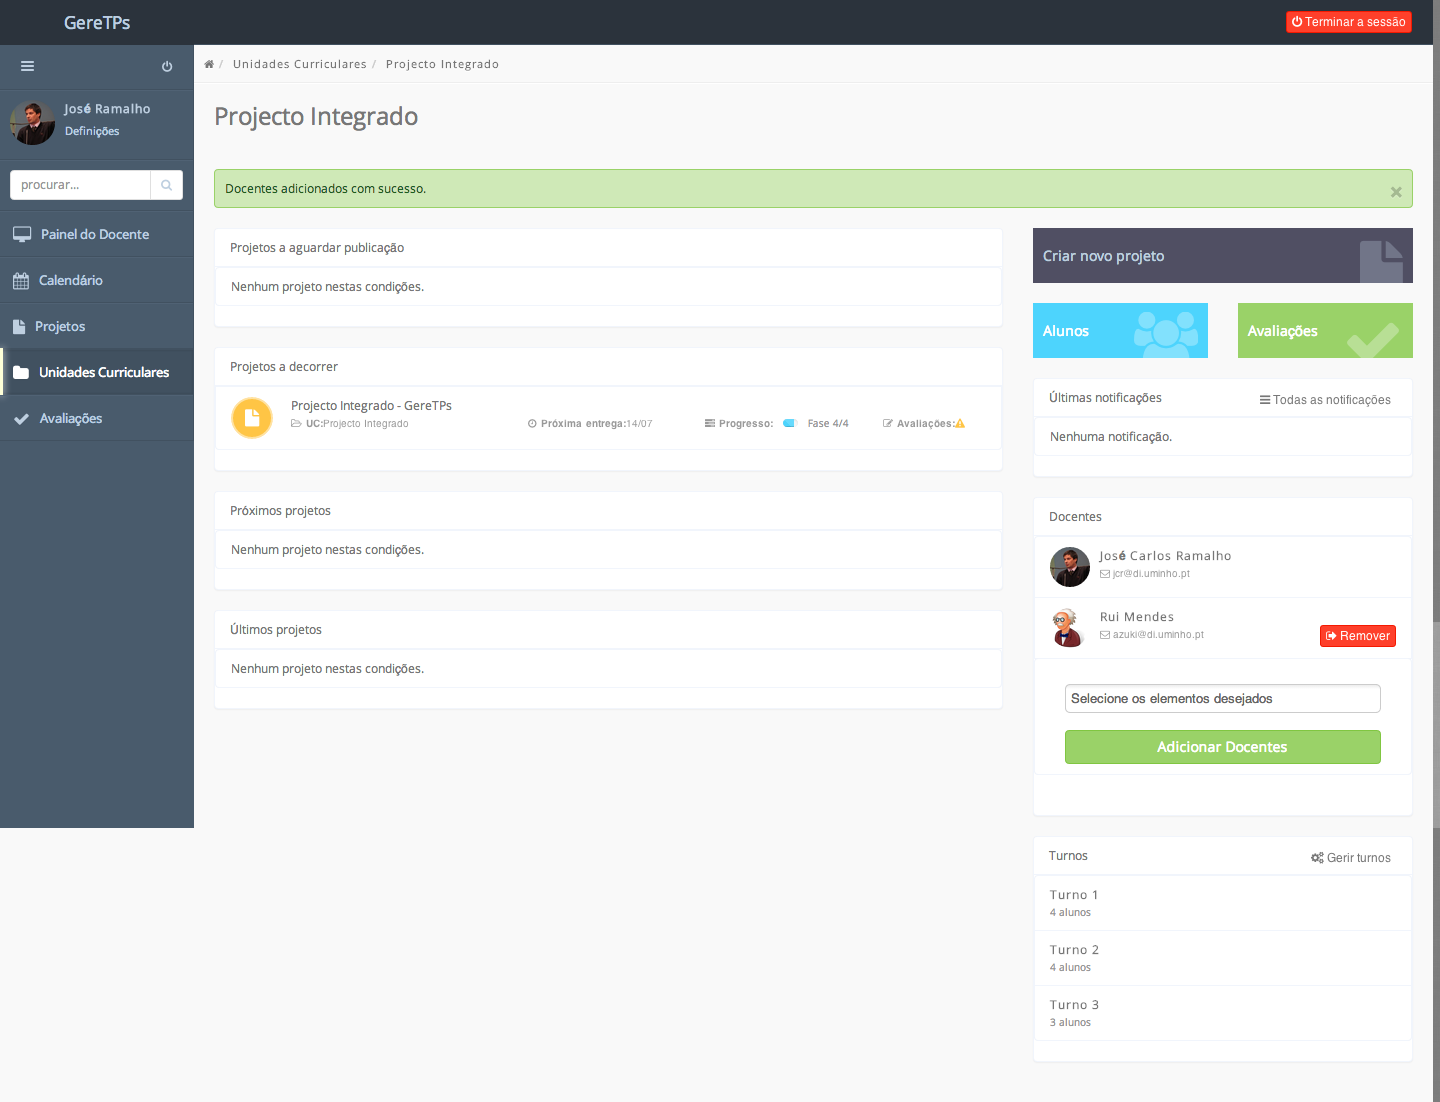
\includegraphics[width=1\textwidth,center]{images/implementacao/docentes/uc}
  \caption{Página de uma unidade curricular}
  \label{fig:teacher_subjects}
\end{figure}
